\problem{}
Run the Ford-Fulkerson algorithm on the flow network in the figure below, and
show the residual network after each flow augmentation. For each iteration, pick
the augmenting path that is lexicographically smallest. (e.g. if you have two
augmenting paths 1 $\rightarrow$ 3 $\rightarrow$ $t$ and 1 $\rightarrow$ 4 $\rightarrow$ $t$, then you should choose 1 $\rightarrow$ 3 $\rightarrow$ $t$, because it is lexicographically smaller than 1 $\rightarrow$ 4 $\rightarrow$ $t$).


\begin{figure}[htbp]
    \centering
    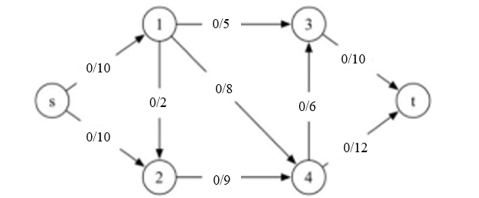
\includegraphics[width=0.8\textwidth]{netflow.png}
    \end{figure} 


\solution{

}
\newpage